\documentclass{beamer}
% Setup for bibliography
\usepackage[
backend=biber,
style=numeric-comp,
]{biblatex}
\addbibresource{../../references.bib}

% Pretty self explanatory
% We sue this in title bits
\usepackage{datetime}

% Standard math packages / setup
\usepackage{amsmath} 
\usepackage{amsfonts}
\usepackage{amsthm}
\usepackage{amssymb} 
\usepackage{accents}
\usepackage{mathrsfs}
\usepackage{mathtools}

\usepackage{bm}

%\newtheorem{lemma}{Lemma}
%\newtheorem{theorem}{Theorem}
%\newtheorem{definition}{Definition}

% So we can import pngs
\usepackage{graphicx} 

% This gives us nice clickable links 
% https://www.overleaf.com/learn/latex/Hyperlinks#Styles_and_colours
\usepackage{hyperref}
\hypersetup{
    colorlinks=true,
    linkcolor=blue,
    citecolor=blue,
    filecolor=magenta,      
    urlcolor=cyan,
    pdftitle={Monte Carlo Methods (DRAFT)},
    pdfpagemode=FullScreen,
    }
\urlstyle{same}

% Allows us to define colors
% We use this in the next block, listings
\usepackage{color}
\definecolor{dkgreen}{rgb}{0,0.6,0}
\definecolor{gray}{rgb}{0.5,0.5,0.5}
\definecolor{mauve}{rgb}{0.58,0,0.82}

% Allows us to include 
\usepackage{listings}
\lstset{frame=tb,
  language={},
  aboveskip=3mm,
  belowskip=3mm,
  showstringspaces=false,
  columns=flexible,
  basicstyle={\small\ttfamily},
  numbers=none,
  numberstyle=\tiny\color{gray},
  keywordstyle=\color{blue},
  commentstyle=\color{dkgreen},
  stringstyle=\color{mauve},
  breaklines=true,
  breakatwhitespace=true,
  tabsize=4
}

% Adds bulletized outlines with outline environment
\usepackage{outlines}

% Tikz
\usepackage{tikz}

% Colors
\usepackage{xcolor}
\definecolor{uconnblue}{rgb}{0.08, 0.18, 0.28}
\definecolor{intactblue}{rgb}{0.13, 0.26, 0.45}
\definecolor{mastercamred}{rgb}{0.83, 0.01, 0.23}

% By default beamer slides are 4:3 , 128mm by 96mm

\logo{
\includegraphics[height=0.5cm]{../../assets/SBU_logos/horz_2clr_rgb_300ppi.png}}

\usetheme{CambridgeUS}

\AtBeginSection[]
{
  \begin{frame}
    \frametitle{Table of Contents}
    \tableofcontents[currentsection]
  \end{frame}
}

% \shadowimage[width=8cm]{image}
%
% Provides a drop-shadow to images
%
% From
% https://tex.stackexchange.com/questions/81842/creating-a-drop-shadow-with-guassian-blur 
\usetikzlibrary{shadows,calc}

% code adapted from https://tex.stackexchange.com/a/11483/3954

% some parameters for customization
\def\shadowshift{3pt,-3pt}
\def\shadowradius{6pt}

\colorlet{innercolor}{black!60}
\colorlet{outercolor}{gray!05}

% this draws a shadow under a rectangle node
\newcommand\drawshadow[1]{
    \begin{pgfonlayer}{shadow}
        \shade[outercolor,inner color=innercolor,outer color=outercolor] ($(#1.south west)+(\shadowshift)+(\shadowradius/2,\shadowradius/2)$) circle (\shadowradius);
        \shade[outercolor,inner color=innercolor,outer color=outercolor] ($(#1.north west)+(\shadowshift)+(\shadowradius/2,-\shadowradius/2)$) circle (\shadowradius);
        \shade[outercolor,inner color=innercolor,outer color=outercolor] ($(#1.south east)+(\shadowshift)+(-\shadowradius/2,\shadowradius/2)$) circle (\shadowradius);
        \shade[outercolor,inner color=innercolor,outer color=outercolor] ($(#1.north east)+(\shadowshift)+(-\shadowradius/2,-\shadowradius/2)$) circle (\shadowradius);
        \shade[top color=innercolor,bottom color=outercolor] ($(#1.south west)+(\shadowshift)+(\shadowradius/2,-\shadowradius/2)$) rectangle ($(#1.south east)+(\shadowshift)+(-\shadowradius/2,\shadowradius/2)$);
        \shade[left color=innercolor,right color=outercolor] ($(#1.south east)+(\shadowshift)+(-\shadowradius/2,\shadowradius/2)$) rectangle ($(#1.north east)+(\shadowshift)+(\shadowradius/2,-\shadowradius/2)$);
        \shade[bottom color=innercolor,top color=outercolor] ($(#1.north west)+(\shadowshift)+(\shadowradius/2,-\shadowradius/2)$) rectangle ($(#1.north east)+(\shadowshift)+(-\shadowradius/2,\shadowradius/2)$);
        \shade[outercolor,right color=innercolor,left color=outercolor] ($(#1.south west)+(\shadowshift)+(-\shadowradius/2,\shadowradius/2)$) rectangle ($(#1.north west)+(\shadowshift)+(\shadowradius/2,-\shadowradius/2)$);
        \filldraw ($(#1.south west)+(\shadowshift)+(\shadowradius/2,\shadowradius/2)$) rectangle ($(#1.north east)+(\shadowshift)-(\shadowradius/2,\shadowradius/2)$);
    \end{pgfonlayer}
}

% create a shadow layer, so that we don't need to worry about overdrawing other things
\pgfdeclarelayer{shadow} 
\pgfsetlayers{shadow,main}


\newcommand\shadowimage[2][]{%
\begin{tikzpicture}
\node[anchor=south west,inner sep=0] (image) at (0,0) {\includegraphics[#1]{#2}};
\drawshadow{image}
\end{tikzpicture}}



%Information to be included in the title page:
\title{Advanced Automatic Code Generation For Multiple Relaxation-Time Lattice Boltzmann Methods}
\author{Frederick Hennig, Markus Holzer, and Ulrich R{\"u}de \\ \vspace{0.5cm} Presented by Russell Bentley}
\institute{Stony Brook}
\date{2024}

\begin{document}

\frame{\titlepage}

 %% Whate are we talking about
\placelogofalse
\begin{frame}{Introduction}
\begin{columns}
\column{0.58\linewidth}
\centering
\begin{outline}
  \1 LBM is a framework for numerically modeling Fluid dynamics
  \1 Historically, not great for turbulence
  \1 New collision operators like CM-MRT improve this
  \1 Adoption for graphics research \cite{Li2020, Li2024, Lyu2021}
\end{outline}

\column{0.38\linewidth}
\begin{center}
\centering
\shadowimage[width=2.5cm]{li2020_image.png}

\shadowimage[width=2.5cm]{lyu2021_image.png} 
\end{center}
\end{columns}
\end{frame}
\placelogotrue

\placelogofalse
\begin{frame}{Results}
  \begin{center}
  \centering
  \includegraphics[width=0.7\linewidth]{result_03.png}

  \includegraphics[width=0.7\linewidth]{stream_03.png}
  \end{center}
\end{frame}
\placelogotrue


%%%
%%% cm_lbm slides
%%%

\placelogofalse
\begin{frame}{Introduction}
\begin{columns}
\column{0.58\linewidth}
\centering
\begin{outline}
  \1 LBM is a framework for numerically modeling Fluid dynamics
  \1 Historically, not great for turbulence
  \1 New collision operators like CM-MRT improve this
  \1 Adoption for graphics research \cite{Li2020, Li2024, Lyu2021}
\end{outline}

\column{0.38\linewidth}
\begin{center}
\centering
\shadowimage[width=2.5cm]{li2020_image.png}

\shadowimage[width=2.5cm]{lyu2021_image.png} 
\end{center}
\end{columns}
\end{frame}
\placelogotrue

\placelogofalse
\begin{frame}{Results}
  \begin{center}
  \centering
  \includegraphics[width=0.7\linewidth]{result_03.png}

  \includegraphics[width=0.7\linewidth]{stream_03.png}
  \end{center}
\end{frame}
\placelogotrue

\begin{frame}{Architecture}
  \begin{center}
  \centering
  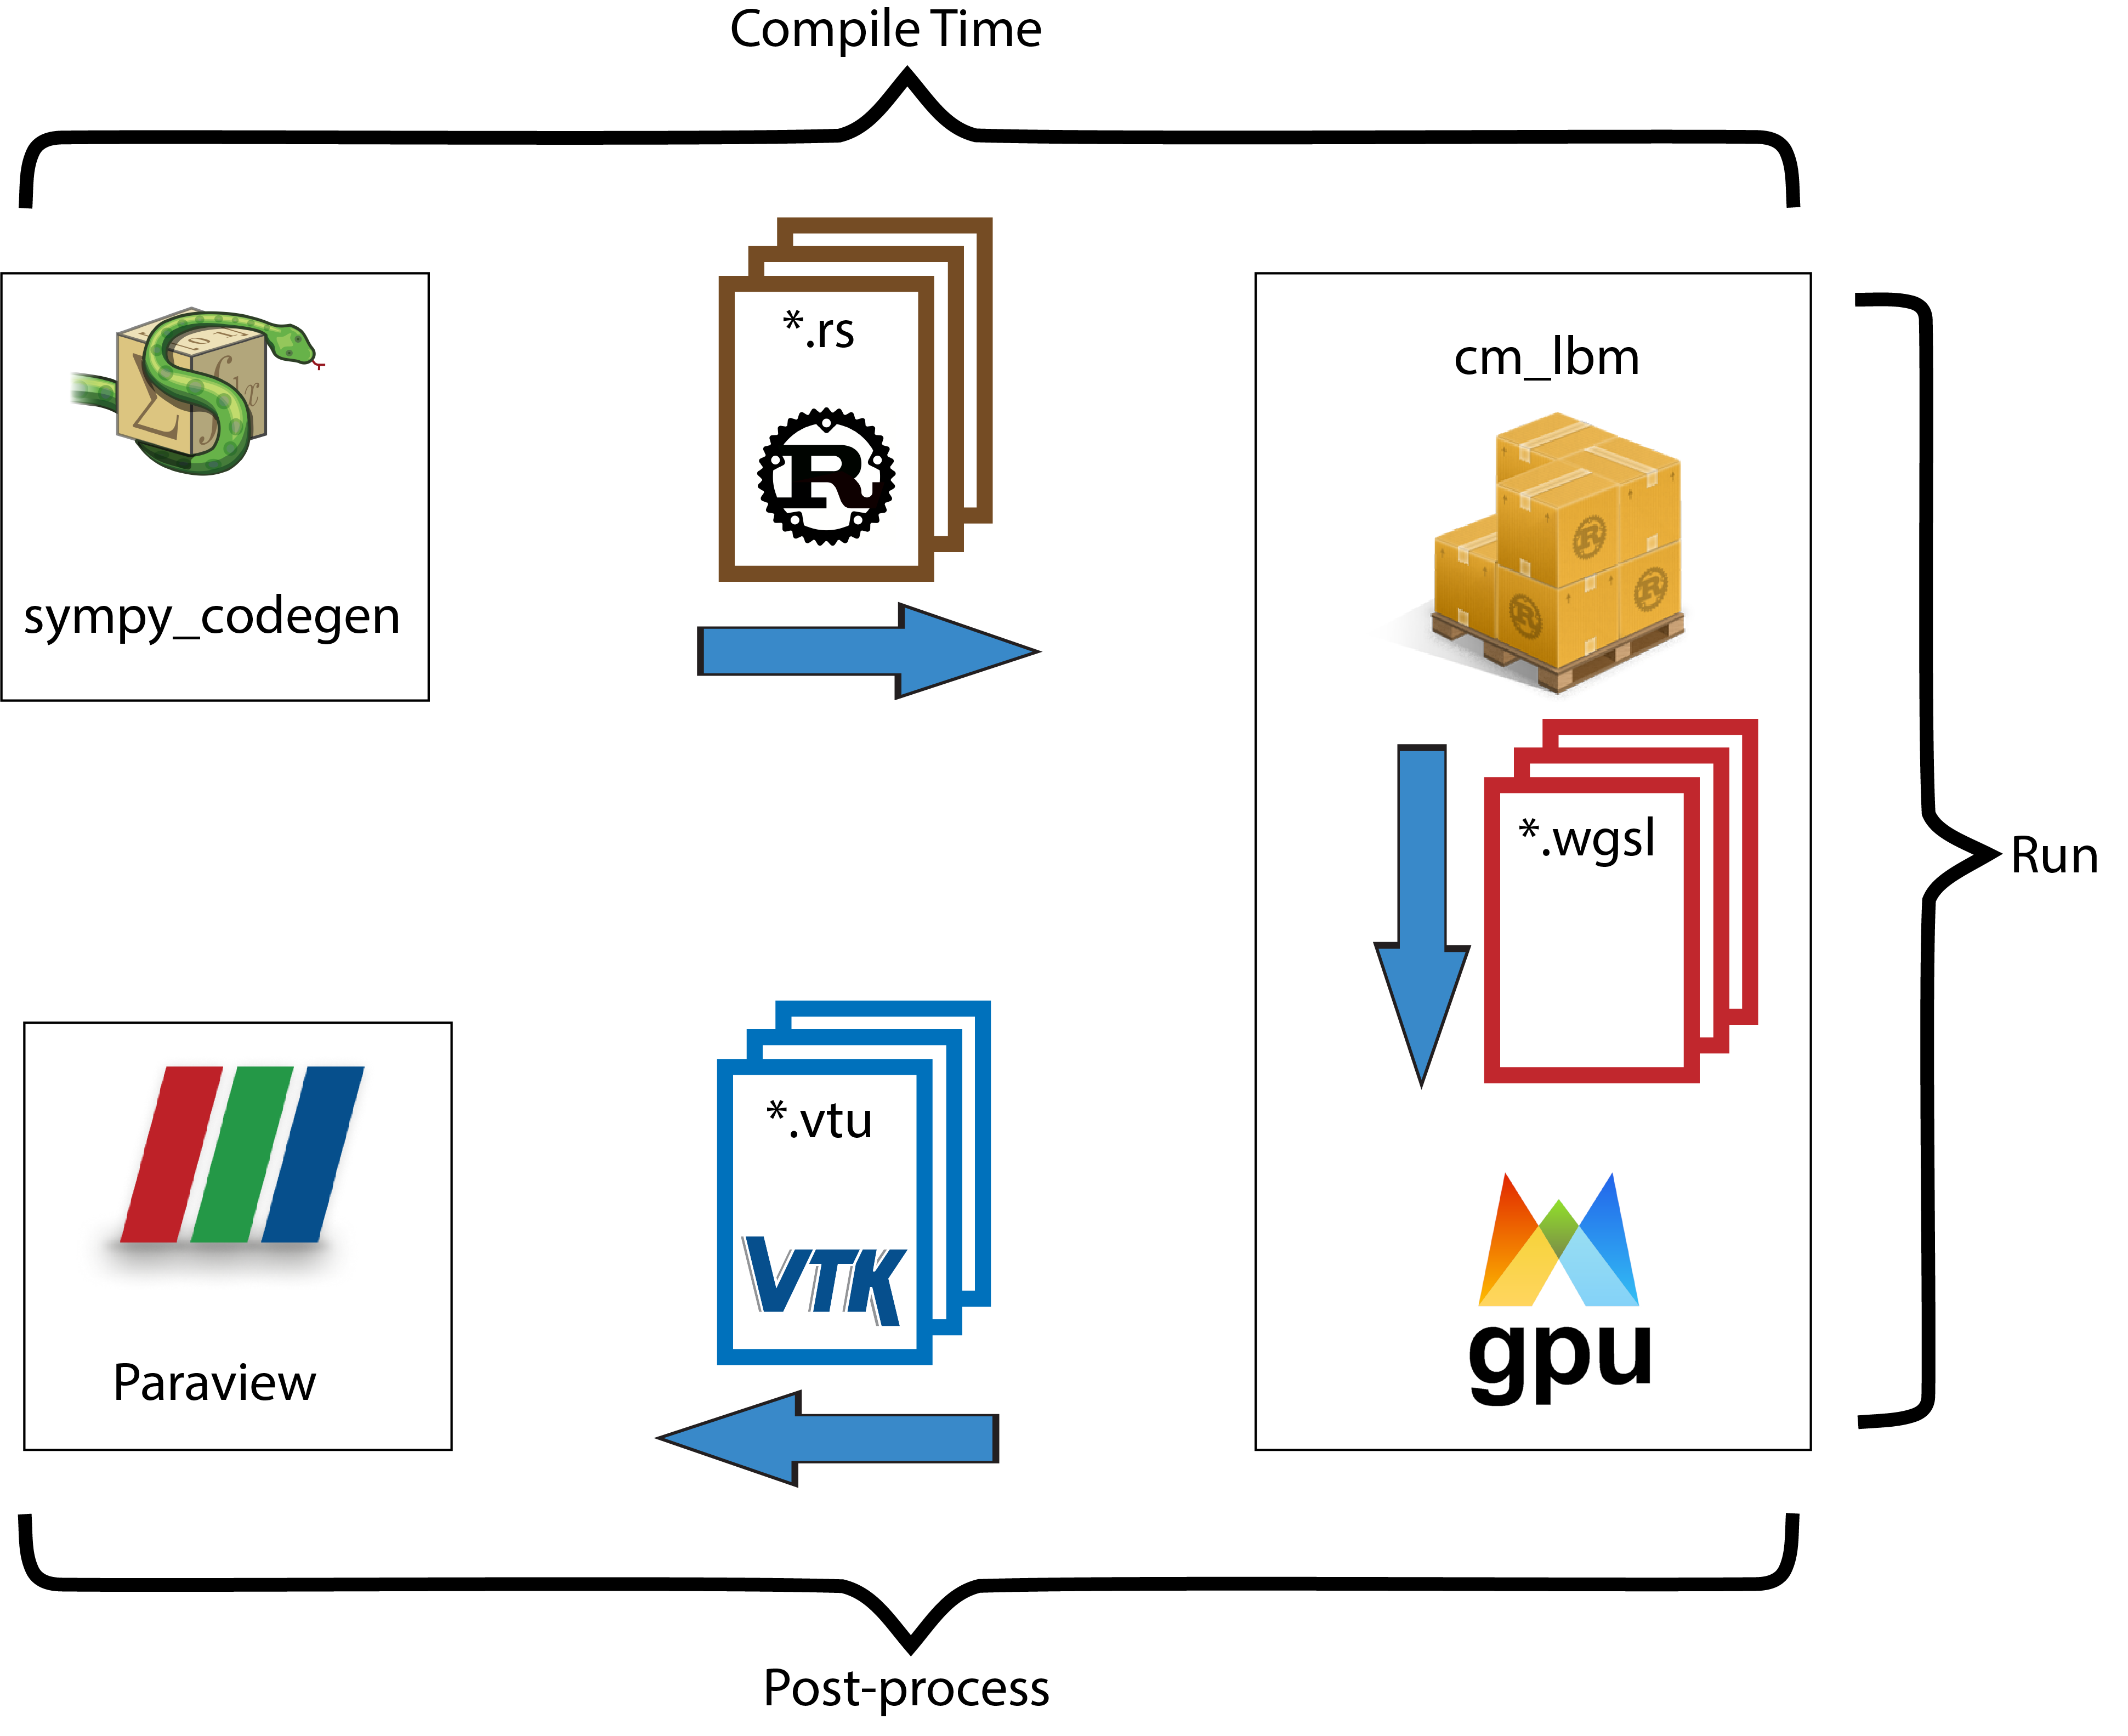
\includegraphics[width=0.7\linewidth]{workflow.png}
  \end{center}
  \blfootnote{\url{https://github.com/SallySoul/lbm3}}
\end{frame}

\begin{frame}{Paraview + VTK}
\begin{center}
\centering
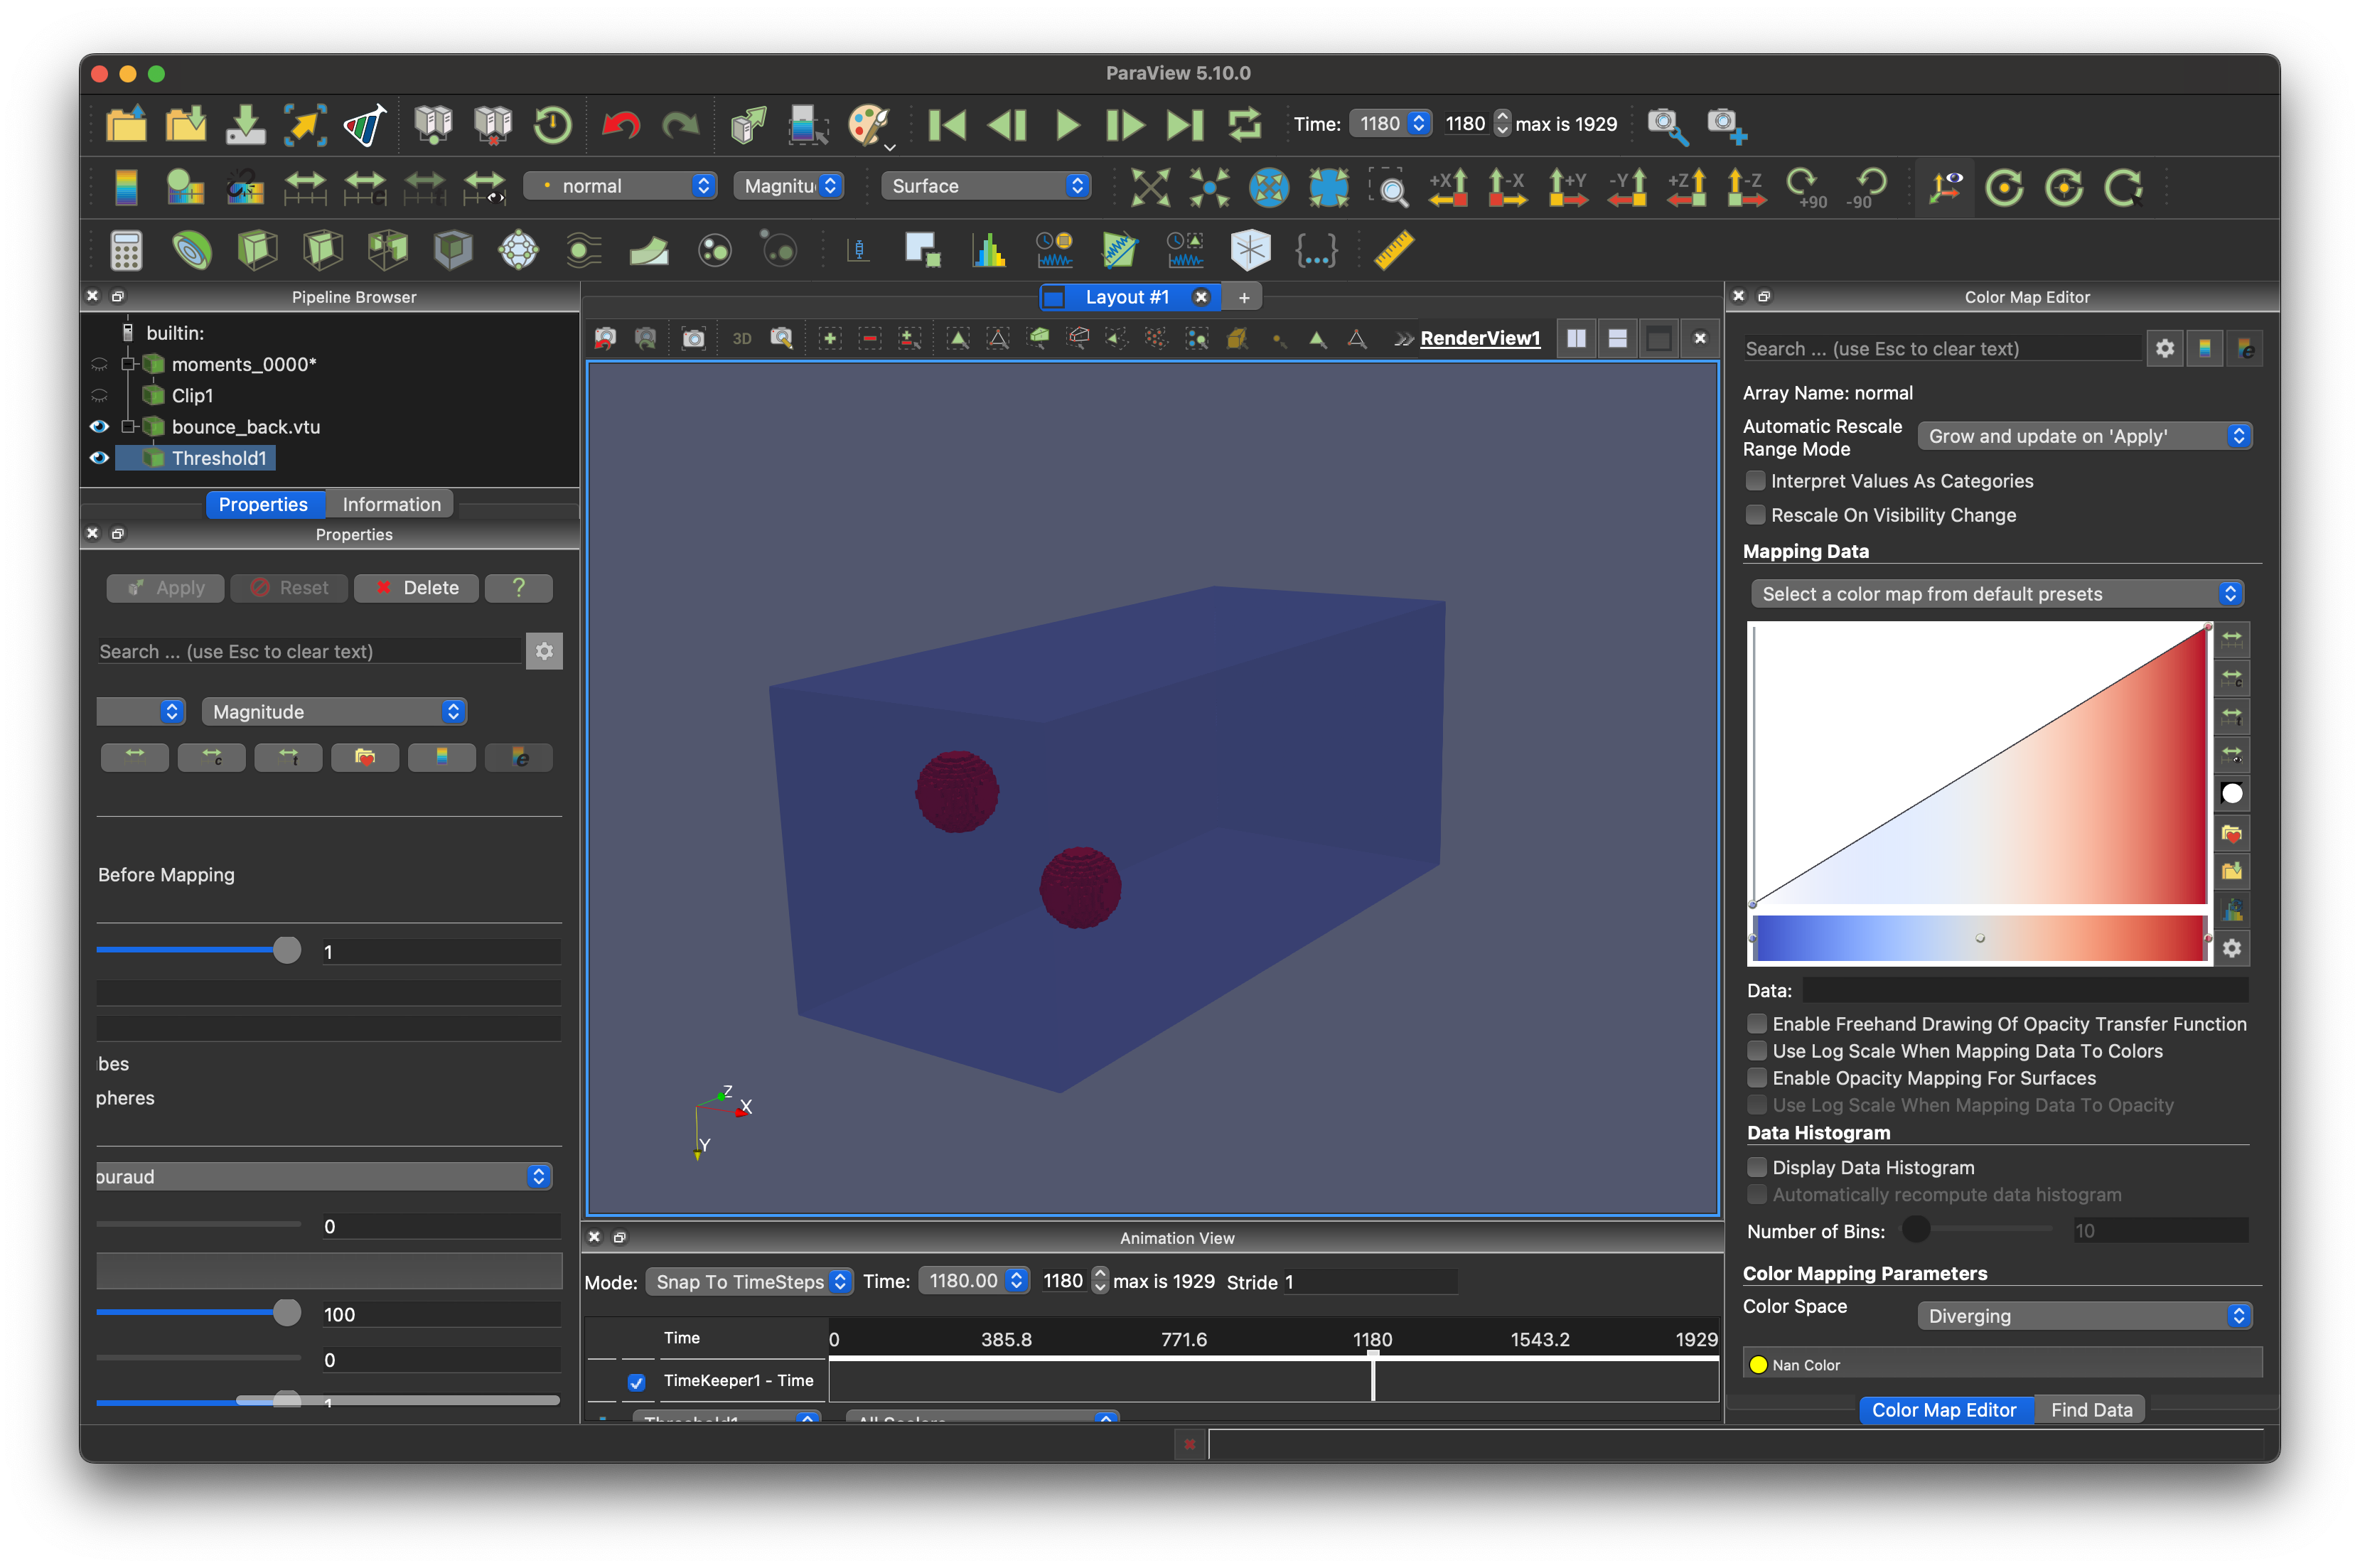
\includegraphics[width=0.7\linewidth]{example_1_paraview.png}
\end{center}
\blfootnote{\url{https://www.paraview.org}}
\blfootnote{\url{https://vtk.org}}
\end{frame}

\placelogofalse
\begin{frame}{Lattice Boltzmann method (LBM)}
\begin{columns}
\column{0.48\linewidth}
\begin{outline}
\1 $D$ dimensional grid of points $x$
\1 Microscopic velocity distribution $f(x, t)$ at each point
\1 $Q$ discrete microscopic velocities $c_i$
\1 Macroscropic properties are moments of microscopic distributions
\1 Advance time with two operators, 
\textit{streaming} and \textit{collision}
\end{outline}

\column{0.48\linewidth}
\centering
\begin{center}
  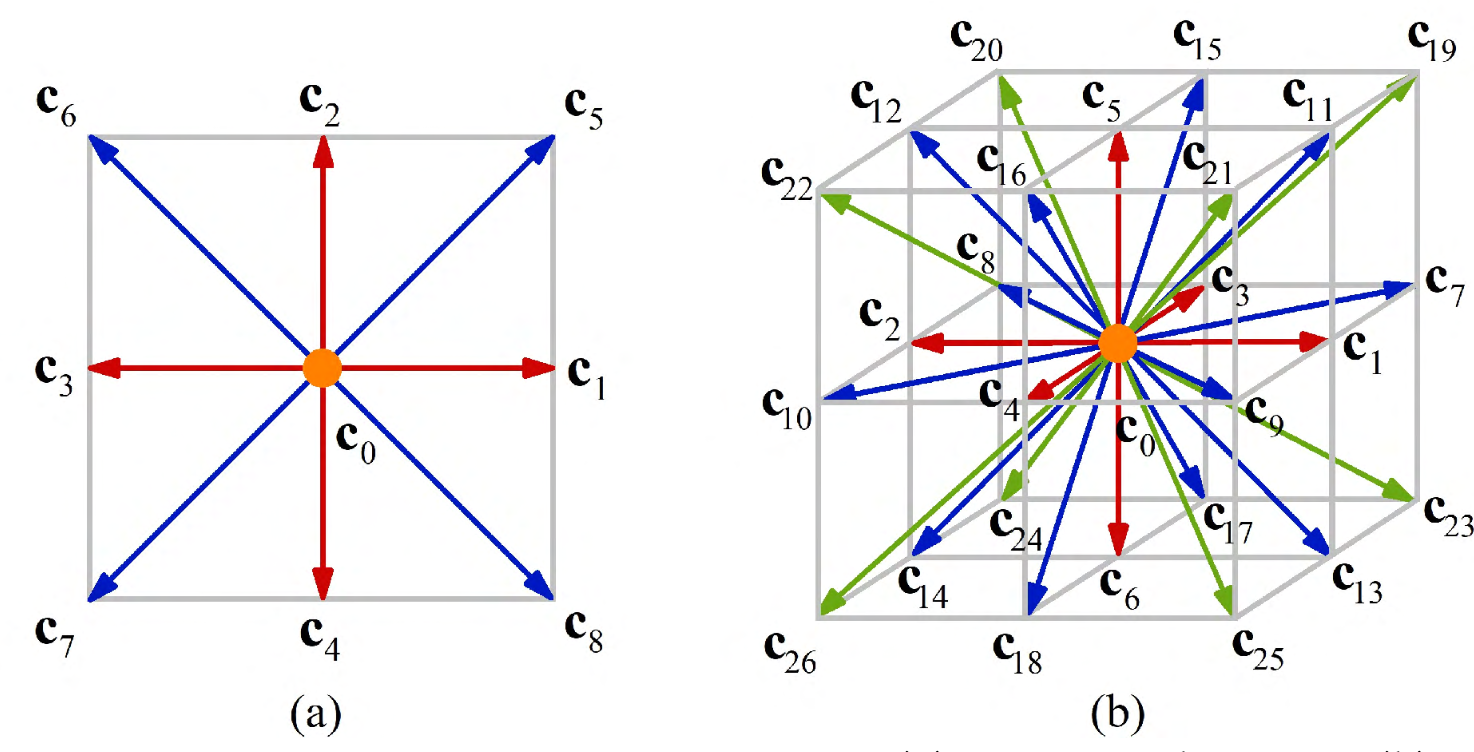
\includegraphics[width=0.9\linewidth]{lattice_figure.png}

  \begin{align*}
  \rho(x, t) &= \sum_{i = 0}^{Q - 1} f_i(x, t) \\
  \rho(x,t)u(x,t) &= \sum_{i = 0}^{Q - 1}c_i f_i(x, t)
  \end{align*}
\end{center}
\end{columns}
\blfootnote{Figure from \cite{Li2020}}
\end{frame}
\placelogotrue

\begin{frame}{Storage and Streaming}
\begin{columns}
\column{0.48\linewidth}
\begin{outline}
\1 Non-local operator
\1 Send velocity distribution to neighbor point
\1 Information travels at speed of sound!
\1 How are distributions stored? (AoS, SoA)
\1 Double buffered?
\end{outline}

\column{0.48\linewidth}
\centering
  \begin{center}
    \includegraphics[width=0.4\linewidth]{stream_0.png}
    \includegraphics[width=0.4\linewidth]{stream_1.png}

    \includegraphics[width=0.6\linewidth]{stream_2.png}
  \end{center}
\end{columns}
\end{frame}



\begin{frame}{Collision (BGK)}
\begin{columns}
\column{0.48\linewidth}
\begin{outline}
\1 Collision is local
\1 Relax distributions towards equilibrium
\1 BGK is standard collision operator
\2 Relaxes all distributions at constant rate
\1 First order approximation
\end{outline}
\column{0.48\linewidth}
\begin{center}
\begin{align*}
    \text{BGK}(f) &= \frac{1}{\tau} (f_{\text{eq}} - f)
\end{align*}
\end{center}
\end{columns}
\vspace{1cm}
\begin{align*}
   f_{\text{eq}} &= w_i \rho \left(
1 + 3 c_i \cdot u  + \frac{9 (c_i \cdot u)^2}{2}
- \frac{3 (u \cdot u)^2}{2}\right) \\
\end{align*}
\end{frame}

\begin{frame}{Multiple Relaxation Time (MRT)}
\begin{columns}
\column{0.48\linewidth}
\begin{outline}
\1 $M$ transforms $f$ into moment space
\1 $26$ of them!
\1 Relax moments separately
\1 $M^{-1}$ transforms result back to distribution
\end{outline}
\column{0.48\linewidth}
\begin{center}
\begin{align*}
m_{0,j} &= \{  1 \},\\
m_{1,j} &= \{  c_{j,x} \}, \\
m_{18,j} &= \{ c_{j,x}^2 c_{j,y}^2 + c_{j,x}^2 c_{j,z}^2 - c_{j,y}^2 c_{j,z}^2 \}, \\
m_{19,j} &= \{ c_{j,x}^2 c_{j,y}^2 - c_{j,x}^2 c_{j,z}^2 \},\\
m_{26,j} &= \{ c_{j,x}^2 c_{j,y}^2 c_{j,z}^2 \},\\
\end{align*}
\end{center}
\end{columns}
\begin{center}
  \begin{align*}
\text{MRT}(f) &= M^{-1} \cdot R \cdot M(f_{\text{eq}} - f)
  \end{align*}
\end{center}
\end{frame}

\begin{frame}{Relaxation Rates, pt 1}
\begin{columns}
\column{0.48\linewidth}
\begin{outline}
\1 Independent relaxation rates for each moment
\1 Zeroth moment, density, should be conserved.
\1 Next three are momentum, $r_i = 2$ is common
\1 Next six moments are related to momentum flux
\2 Relaxation rate is related to viscosity, $v$ 
\end{outline}
\column{0.48\linewidth}
\begin{center}
\begin{align*}
  R &= \left[\begin{array}{c c c c}
  r_0 & 0 & \cdots & 0 \\
  0 & r_1 & \cdots & 0 \\
  \vdots & & & \vdots \\
  0 & & \cdots & r_{26} \\
  \end{array}\right] \\
  r_0 &= 0, \\
  r_i &= 2, \text{ for } i = 1, 2, 3 \\
  r_i &= (3v + 1/2)^{-1}, \text{ for } i = 4,\cdots,9
\end{align*}
\end{center}
\end{columns}
\end{frame}

\begin{frame}{Relaxation Rates, pt 2}
\begin{columns}
\column{0.48\linewidth}
\begin{outline}
\1 Higher-order relaxation rates are an area of active research
\1 \cite{Li2020} Describes an adaptive approach
\1 I implemented fixed rates as described in \cite{Li2018}.
\end{outline}
\column{0.48\linewidth}
\begin{center}
\begin{align*}
  R &= \left[\begin{array}{c c c c}
  r_0 & 0 & \cdots & 0 \\
  0 & r_1 & \cdots & 0 \\
  \vdots & & & \vdots \\
  0 & & \cdots & r_{26} \\
  \end{array}\right] \\
  r_i &= (3v_i + 1 / 2)^{-1}\\
  v_i &= 0.005, \text{ for } i = 9,\ldots, 16 \\
  v_i &= 0.007, \text{ for } i = 17, \ldots, 22 \\
  v_i &= 0.009, \text{ for } i = 26 
\end{align*}
\end{center}
\end{columns}
\end{frame}


\placelogofalse
\begin{frame}{Central Moment MRT (CM-MRT)}
\begin{columns}
\column{0.48\linewidth}
\begin{outline}
\1 MRT violates Galilean invariance 
\2 $u$ changes collision outcome
\1 Center Moments on $u$ \cite{De2017}
\1 $\bar{m}_{\rho} = M_u f_{eq}(u, \rho)$
\2 Equilibrium in CM space
\2 Only depends on $\rho$!
\end{outline}
\column{0.48\linewidth}
\begin{center}
\begin{align*}
\bar{c}_j &= c_j - u \\
m_{0,j} &= \{  1 \},\\
m_{1,j} &= \{  \bar{c}_{j,x} \}, \\
m_{18,j} &= \{ \bar{c}_{j,x}^2 \bar{c}_{j,y}^2 + \bar{c}_{j,x}^2 \bar{c}_{j,z}^2 - \bar{c}_{j,y}^2 \bar{c}_{j,z}^2 \}, \\
m_{19,j} &= \{ \bar{c}_{j,x}^2 \bar{c}_{j,y}^2 - \bar{c}_{j,x}^2 \bar{c}_{j,z}^2 \},\\
m_{26,j} &= \{ \bar{c}_{j,x}^2 \bar{c}_{j,y}^2 \bar{c}_{j,z}^2 \},\\
\end{align*}
\end{center}
\end{columns}
\begin{center}
  \begin{align*}
\text{CM-MRT}_{u,\rho}(f) &= M_u^{-1} \cdot R \cdot (\bar{m}_{\rho} - M_u f)
\end{align*}
\end{center}
\end{frame}
\placelogotrue

\placelogofalse
\begin{frame}{Central Moment MRT (CM-MRT)}
\begin{columns}
\column{0.48\linewidth}
\begin{outline}
\1 MRT violates Galilean invariance 
\1 Center Moments on $u$ \cite{De2017}
\1 $f_{\text{eq}}$ only depends on $\rho$ in CM space
\end{outline}
\column{0.48\linewidth}
\begin{center}
\begin{align*}
\bar{c}_j &= c_j - u \\
m_{0,j} &= \{  1 \},\\
m_{1,j} &= \{  \bar{c}_{j,x} \}, \\
m_{18,j} &= \{ \bar{c}_{j,x}^2 \bar{c}_{j,y}^2 + \bar{c}_{j,x}^2 \bar{c}_{j,z}^2 - \bar{c}_{j,y}^2 \bar{c}_{j,z}^2 \}, \\
m_{19,j} &= \{ \bar{c}_{j,x}^2 \bar{c}_{j,y}^2 - \bar{c}_{j,x}^2 \bar{c}_{j,z}^2 \},\\
m_{26,j} &= \{ \bar{c}_{j,x}^2 \bar{c}_{j,y}^2 \bar{c}_{j,z}^2 \},\\
\end{align*}
\end{center}
\end{columns}
\begin{center}
  \begin{align*}
\text{CM-MRT}_{u,\rho}(f) &= M_u^{-1} \cdot R \cdot (\bar{m}_{\rho} - M_u f)
\end{align*}
\end{center}
\end{frame}
\placelogotrue

\begin{frame}{Code Example: SymPy}
  \begin{center}
  \begin{align*}
  f^{*}_i = f_i + \Omega_i(f, \rho, u).
  \end{align*}
  \shadowimage[width=0.46\linewidth]{bgk_python_code.png}
  \shadowimage[width=0.46\linewidth]{python_code.png}
  \begin{outline}
    \1 Using SymPy was inspired by \cite{Hennig2023}
    \1 Looks like a compiler
  \end{outline}
  \end{center}
\end{frame}

\begin{frame}{Code Example: Shader}
  \begin{center}
  \shadowimage[width=0.6\linewidth]{shader_code.png}
  \end{center}
  \begin{outline}
    \1 $\approx 5$kb for moments shader
    \1 $1.1$mb for CM-MRT shader
    \1 Cheap to compute
    \1 Challenging to debug
  \end{outline}
\end{frame}

\begin{frame}{Code Example: Rust}
  \begin{center}
  \shadowimage[width=0.6\linewidth]{rust_code.png}
  \end{center}
  \begin{outline} 
    \1 With formatting, $\approx 45$k lines
    \1 Easier to test and debug
    \1 Tricky parts match shader exactly
\end{outline}
\end{frame}




% Graphicsfinal conclusion
\begin{frame}{Graphics Final Conclusion}
  \begin{outline}
    \1 How are we feeling about the paper title?
    \2 MRT Lattice Boltzmann methods?
    \2 Code generation using \lstinline{sympy}?
    \1 LBM + \lstinline{sympy}
      \2 \href{http://literatelb.org}{``A Literate Lattice Boltzmann Code''}\cite{web:literate_lbm}
  \end{outline}
  \begin{center}
    
\includegraphics[width=0.8\linewidth]{title_header.png}
  \end{center}
\end{frame}


%%
%% Paper Slides
%%

% Background Projects
\begin{frame}{Paper Context}
  \begin{columns}
  \column{.58\linewidth}
  \begin{outline}
    \1 Today's paper is part of a series
    \1 Collaborative HPC work at German University
    \2 \href{https://www.fau.eu}{Fridrich-Alexander-Universit{\"a}t}
    \1 Also part of \href{https://www.multixscale.eu}{MultiXScale}
    \2 European joint effort on exascale simulation
  \end{outline}

  \column{0.38\linewidth}
  \centering

  \begin{center}
    
\includegraphics[width=4cm]{fau_logo.png}

    \vspace{1cm}

    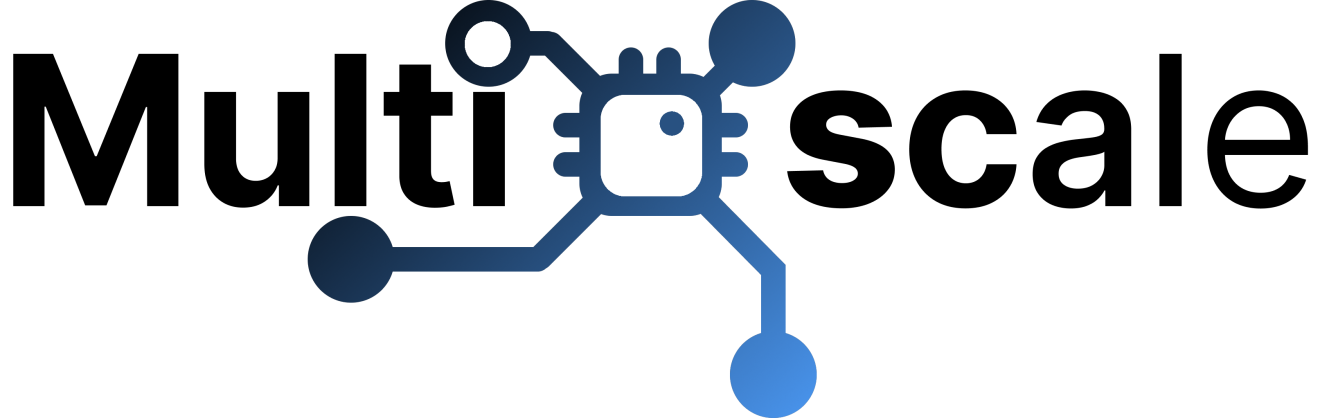
\includegraphics[width=4cm]{multixscale_logo.png}
  \end{center}
\end{columns}
\end{frame}

\placelogofalse
\begin{frame}{waLBerla}
\begin{columns}
\column{0.48\linewidth}
\begin{outline}
  \1 waLBerla framework 
  \2 Introduced in \cite{Bauer2021} (2021)
  \2 HPC-scale simulations
  \2 Stencil problems specifically
  \2 Bring your Compute Kernels
  \1 Provides:
  \2 Multi-node domain partitioning
  \2 Communication patterns 
  \2 Checkpoints
\end{outline}
\column{0.48\linewidth}
\begin{center}
  \shadowimage[width=0.8\linewidth]{juwels.png}
  \vspace{0.5cm}
  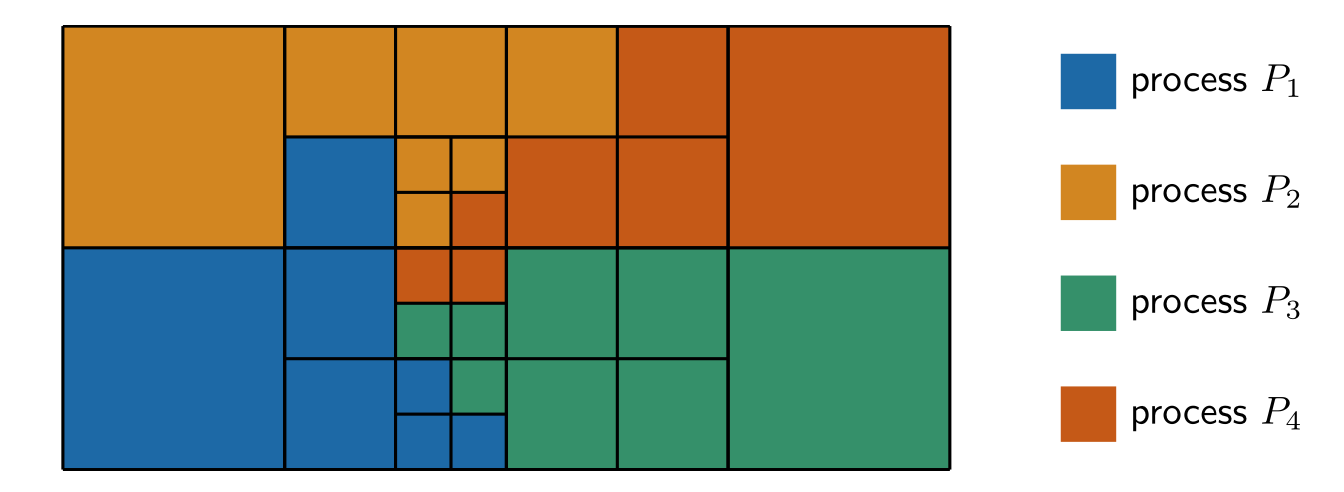
\includegraphics[width=0.8\linewidth]{walberla_partition.png}
  \vspace{0.5cm}
  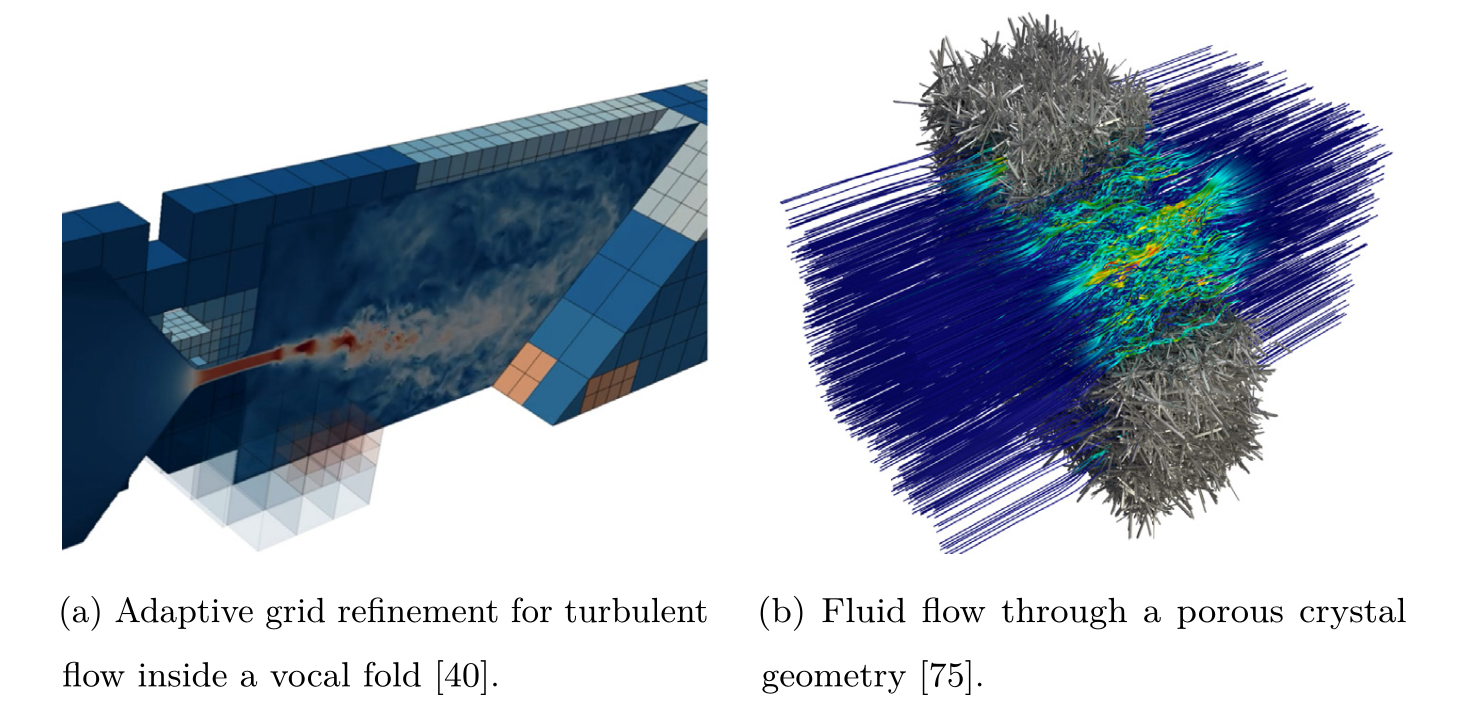
\includegraphics[width=0.8\linewidth]{walberla_examples.png}
\end{center} 
\end{columns}
\blfootnote{From \href{t}{TODO}, \cite{Bauer2021}}
\end{frame}
\placelogotrue


\begin{frame}{\lstinline{pystencils}}
\begin{columns}
  \column{0.48\linewidth}
  \begin{outline}
  \1 Introduced in 2019 \cite{Bauer2019}
  \1 Stencil Compiler 
  \2 \lstinline{sympy}

  \2 Generates optimized compute Kernels
  \2 Introduced in \cite{Bauer2021} (2020)
  \end{outline}

  \column{0.48\linewidth}
  \centering
  \begin{center}
    
\includegraphics[width=0.2\linewidth]{pystencils_logo.png}
  \end{center}
\end{columns}
\end{frame}

\begin{frame}{\lstinline{lbmpy}}
  \begin{columns}
  \column{0.48\linewidth}
  \begin{outline}
  \1 Python package for LBM
  \2 Introduced in \cite{Bauer2021} (2020)
  \end{outline}

  \column{0.48\linewidth}
  \centering
  \begin{center}
    
\includegraphics[width=0.2\linewidth]{lbmpy_logo.png}
  \end{center}
\end{columns}
\end{frame}


% Paper intro
\placelogofalse
\begin{frame}{Introduction}
\begin{columns}
\column{0.48\linewidth}
\begin{outline}
  \1 Presenting \cite{Hennig2023} (2023)
  \2 Adds multiple MRT methods to \lstinline{lbmpy}
  \2 Supports ``arbitrary'' governing eqns
\end{outline}
\column{0.48\linewidth}
\begin{center}
  \shadowimage[width=0.5\linewidth]{hennig_paper.png}

  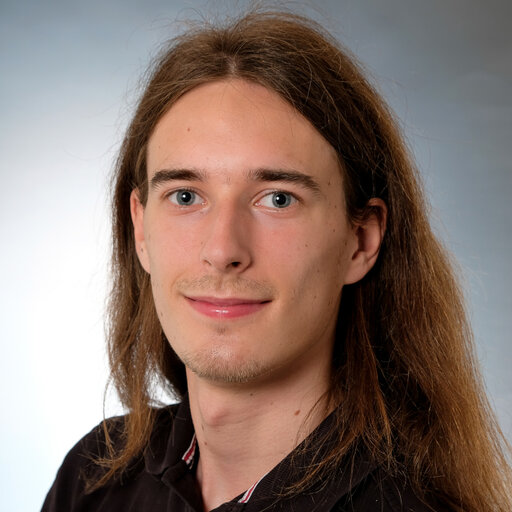
\includegraphics[width=0.3\linewidth]{frederik_hennig.jpg}
  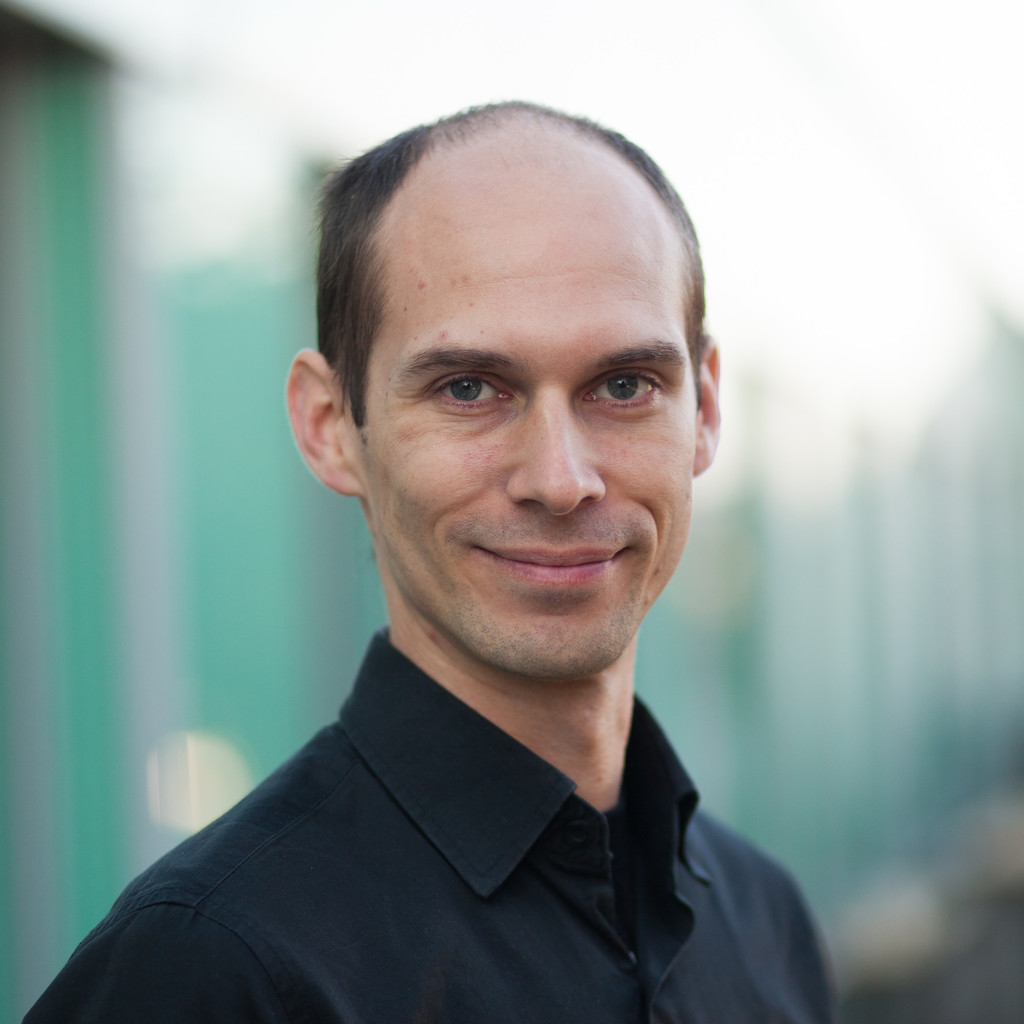
\includegraphics[width=0.3\linewidth]{markus_holzer.jpg}

  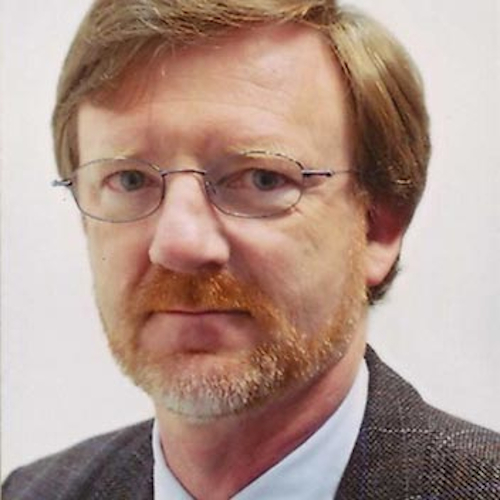
\includegraphics[width=0.3\linewidth]{ulrich_rude.jpg}
\end{center} 
\end{columns}
\end{frame}
\placelogotrue



% Zero-centered
\begin{frame}{Zero-centered Storage}
TODO
\end{frame}


% TODO Simplication Passes 
\placelogofalse
\begin{frame}{Moments}
\begin{columns}
\column{0.48\linewidth}
\begin{center}
\begin{outline}
\1 Capture integral properties of mass density field
\2 Project onto polynomial basis, $b_i$
\end{outline}
\end{center}

\column{0.48\linewidth}
\begin{center}
  \textbf{Moment}
  $$
  M_{i,j,k} = \int_{\Omega} x^i y^j z^k \rho d\Omega
  $$
  Where $i, j, k \in \{0, 1, 2, \cdots\}$

  \vspace{1.5cm}

  \textbf{Moment Vector}
  \begin{align*}
    \bf{M} &= [M_{0,0,0}, M_{1, 0, 0},\\
      & \cdots, M_{n, 0, 0}, M_{n, 1, 0},\\
      & \cdots, M_{n, n, 0}, M_{n, n, 1},\\
      & \cdots, M_{n,n,n}]^T
  \end{align*}
\end{center}
\end{columns}
\end{frame}
\placelogotrue

\begin{frame}{Quadrature From Moments}
We can approximate an integrand f with weighted basis functions.
$$
f \approx \sum_{i = 1}^n c_i b_i
$$
Then by linearity of integrals
$$
\int_{\Omega} f d\Omega \approx \int_{\Omega} \sum_{i = 1}^n c_i b_i \ d \Omega
= \sum_{i=1}^n c_i \int_{\Omega} b_i \ d \Omega
$$
Where $m_i = \int_{\Omega} f_i d \Omega$
\end{frame}

\begin{frame}{Moment Fitting for Quadrature Rules}
\centering
\begin{center}
$$
\bf{A} \cdot \bf{W} = \bf{M}
$$
Where
$$
\bf{A} = \left[
\begin{array}{cccc}
  b_1(x_1) & b_1(x_2) & \cdots & b_1(x_q) \\
  b_2(x_1) & b_2(x_2) & \cdots & b_2(x_q) \\
  \vdots & \vdots & \ddots & \vdots \\
  b_n(x_1) & b_n(x_2) & \cdots & b_n(x_q) \\
\end{array}\right],
W = \left[
  \begin{array}{c}
    w_1 \\ w_2 \\ \vdots \\ w_q
  \end{array}
\right],
M = \left[
  \begin{array}{c}
    m_1 \\ m_2 \\ \vdots \\ m_q
  \end{array}
\right],
$$
With $m_i = \int_{\Omega} b_i \ d\Omega$
\end{center}
\end{frame}

\begin{frame}{Compress Quadrature}
  \centering
  \begin{center}
    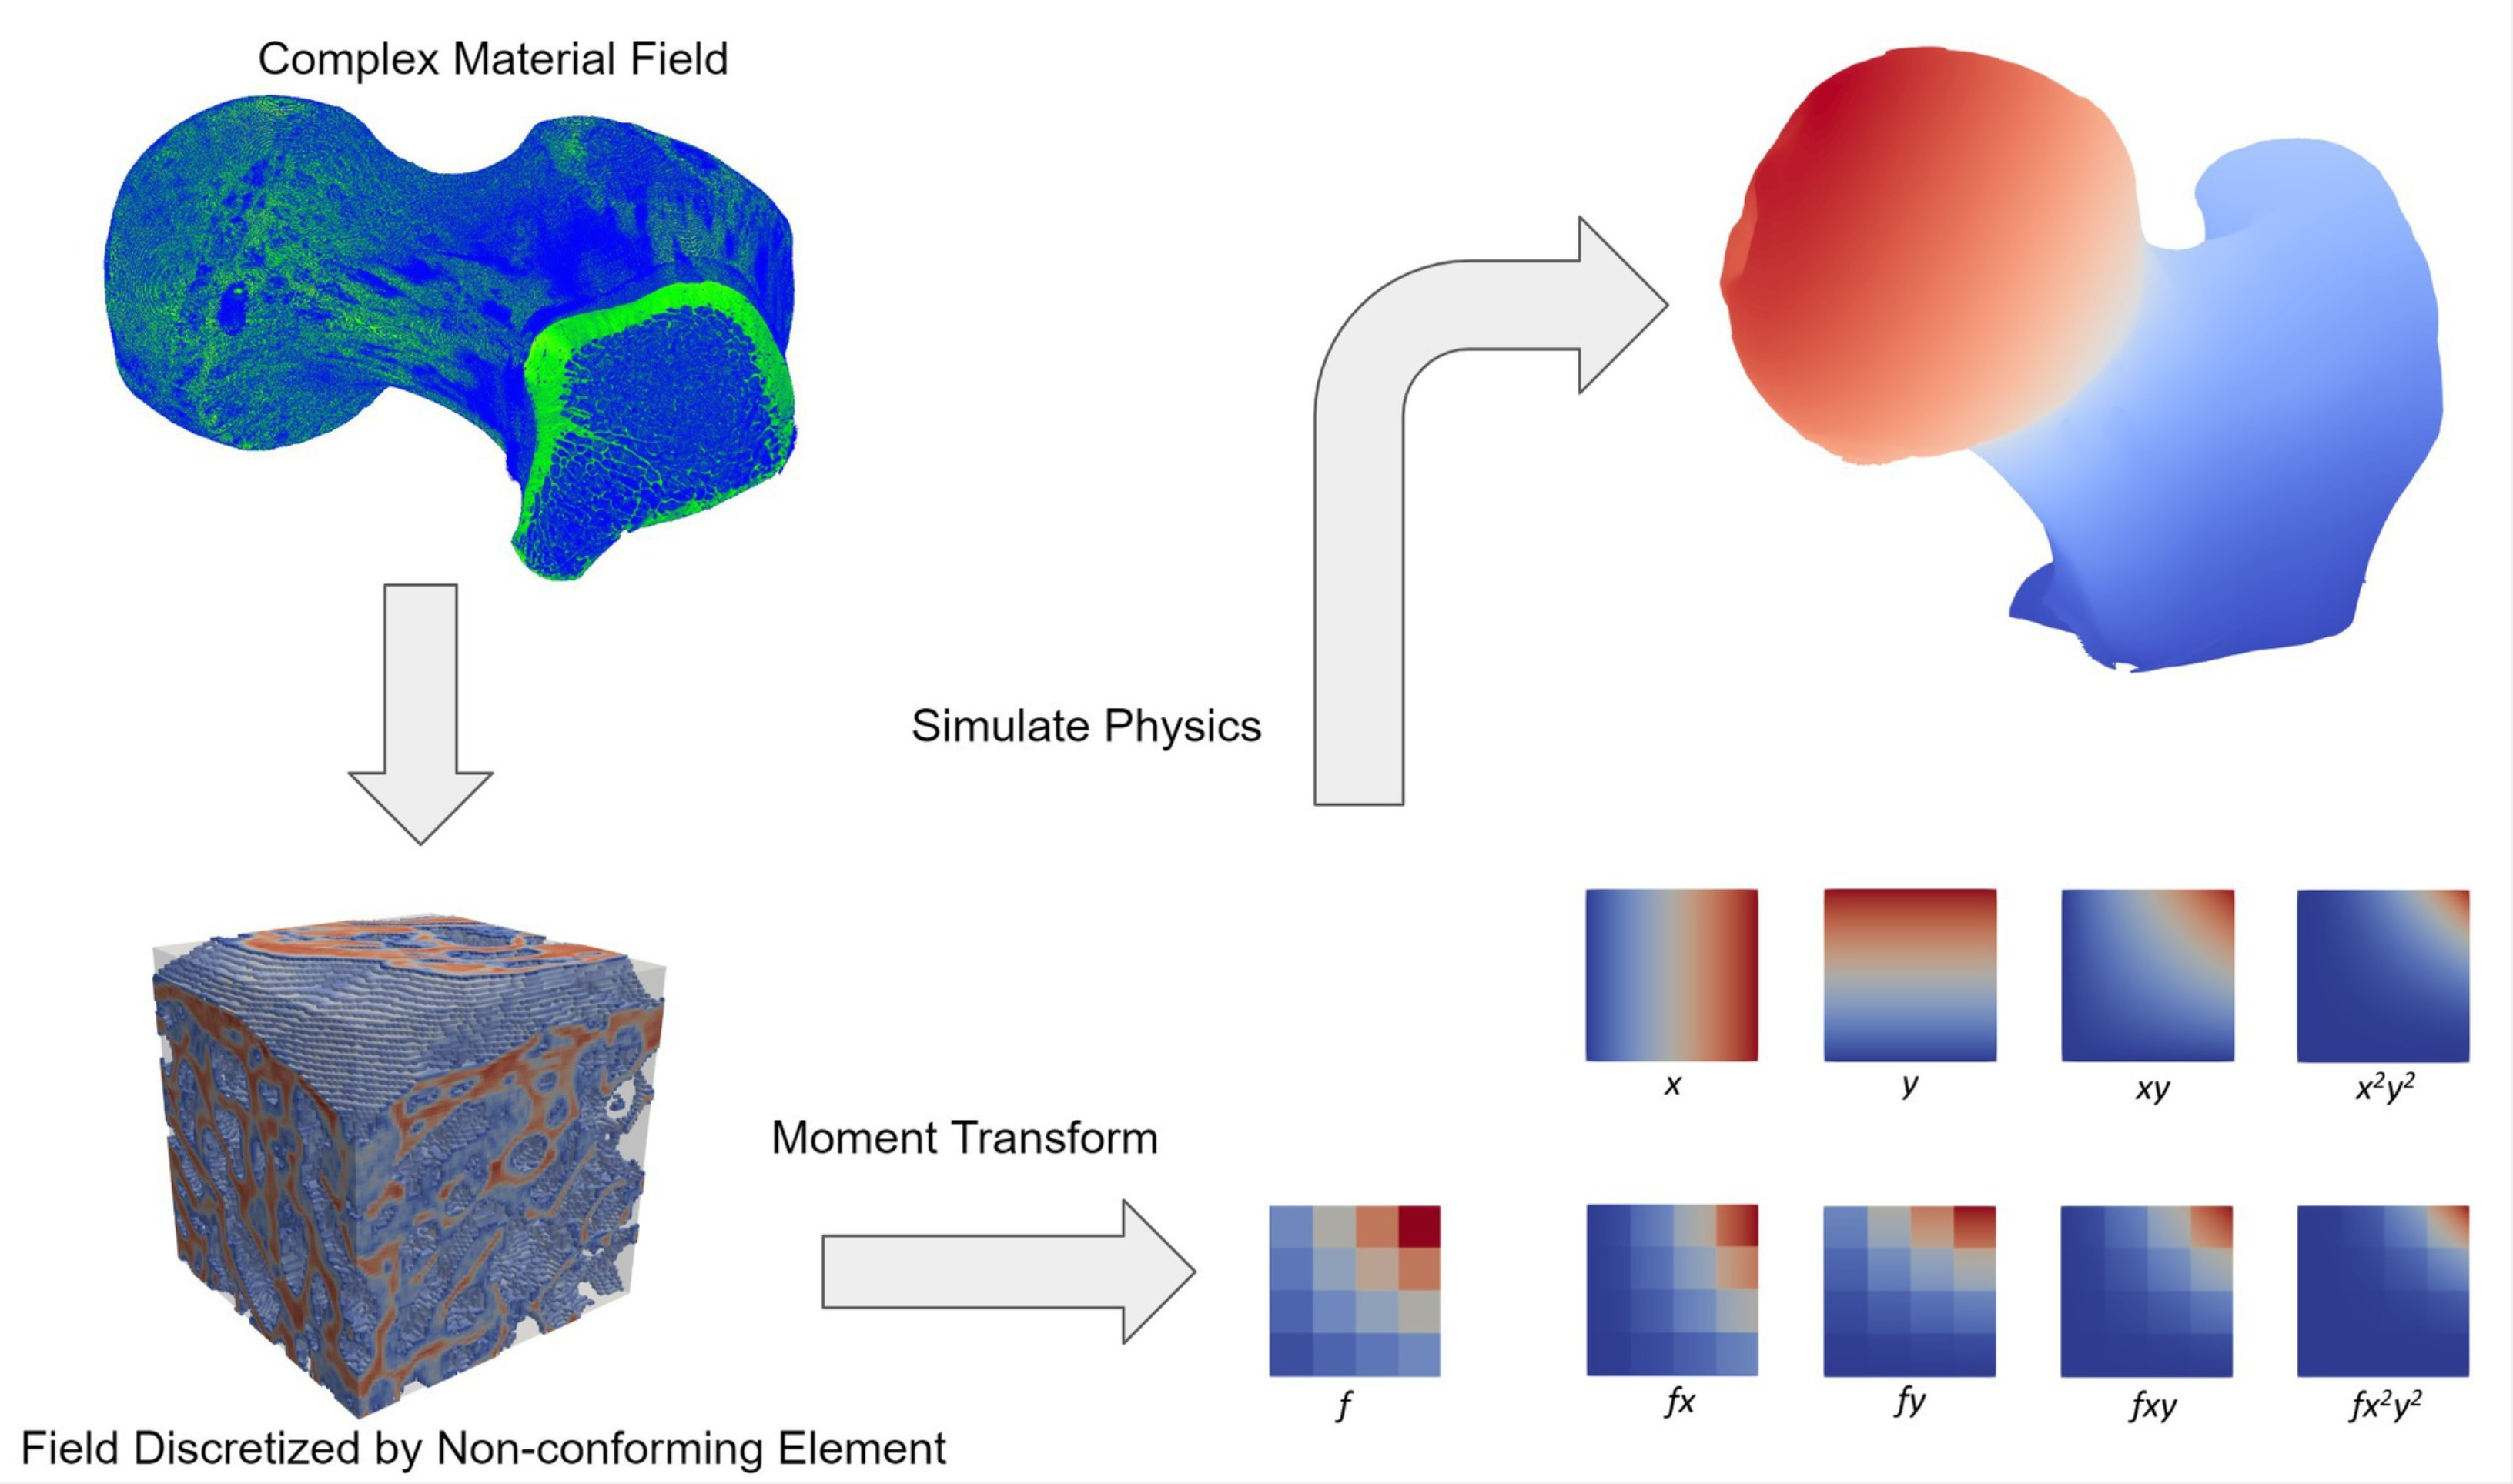
\includegraphics[width=0.8\linewidth]{bone_scan_example.png}\\
  \end{center}
    \blfootnote{Image from \cite{Taber2018}}
\end{frame}

\begin{frame}{Using the Divergence Theorem}
  \begin{center}
    \shadowimage[width=0.6\linewidth]{GeometryCell_scene_1.png}

    \shadowimage[width=0.3\linewidth]{GeometryCell_whole_1.png}
    \shadowimage[width=0.3\linewidth]{GeometryCell_outline_1.png}
  \end{center}
\end{frame}


\begin{frame}{Consequences}
\begin{columns}
\column{0.58\linewidth}
  \begin{outline}
    \1 Generalizes from just density to other fields like conductivity or even stiffness (spatially variable materials)
    \1 This was my job, shuttling data where it needs to be
  \end{outline}
\column{0.38\linewidth}
\begin{center}
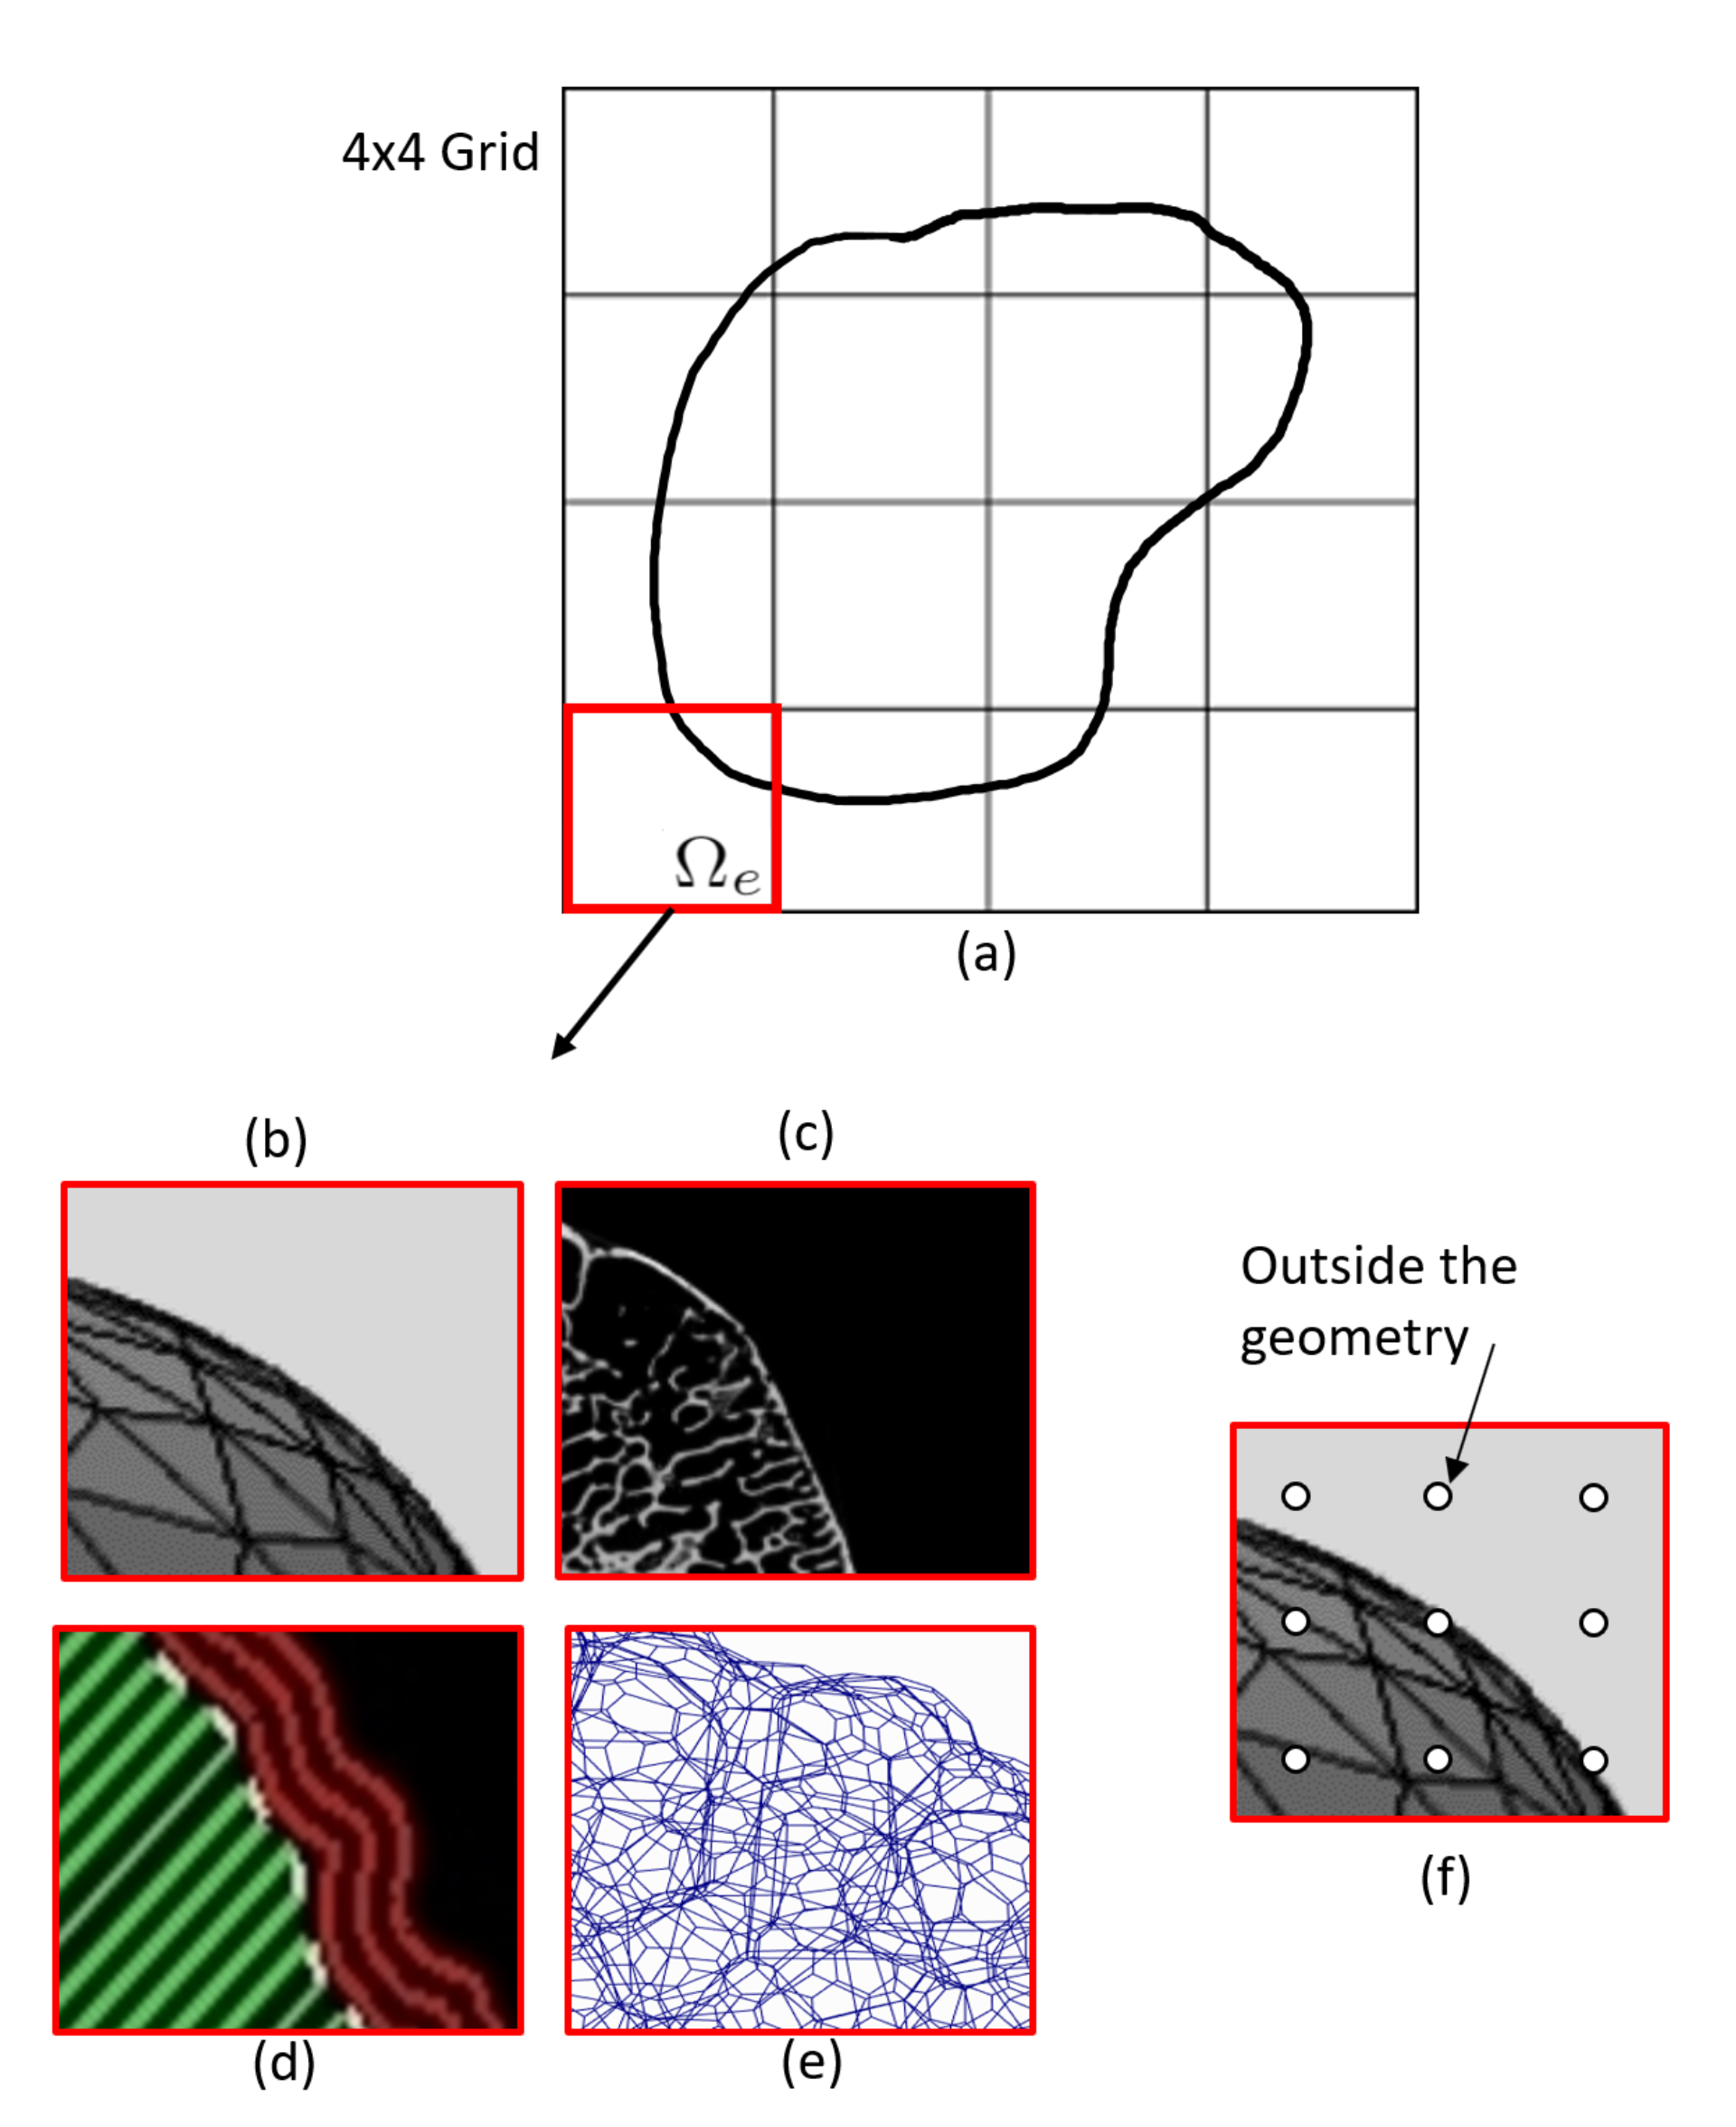
\includegraphics[width=4cm]{immersed_moments.png} 
\end{center}
\end{columns}
\blfootnote{Image from \cite{Taber2018}}
\end{frame}


\begin{frame}{Simplification Passes}
TODO
\end{frame}

% "Operation Count"
% rg '\+|\*|\-' cm_lbm_generated/src/shader_ops/cm_mrt.rs -o  | wc -l
\begin{frame}{Symbolic Simplification Results}
  \centering
  \begin{center}
    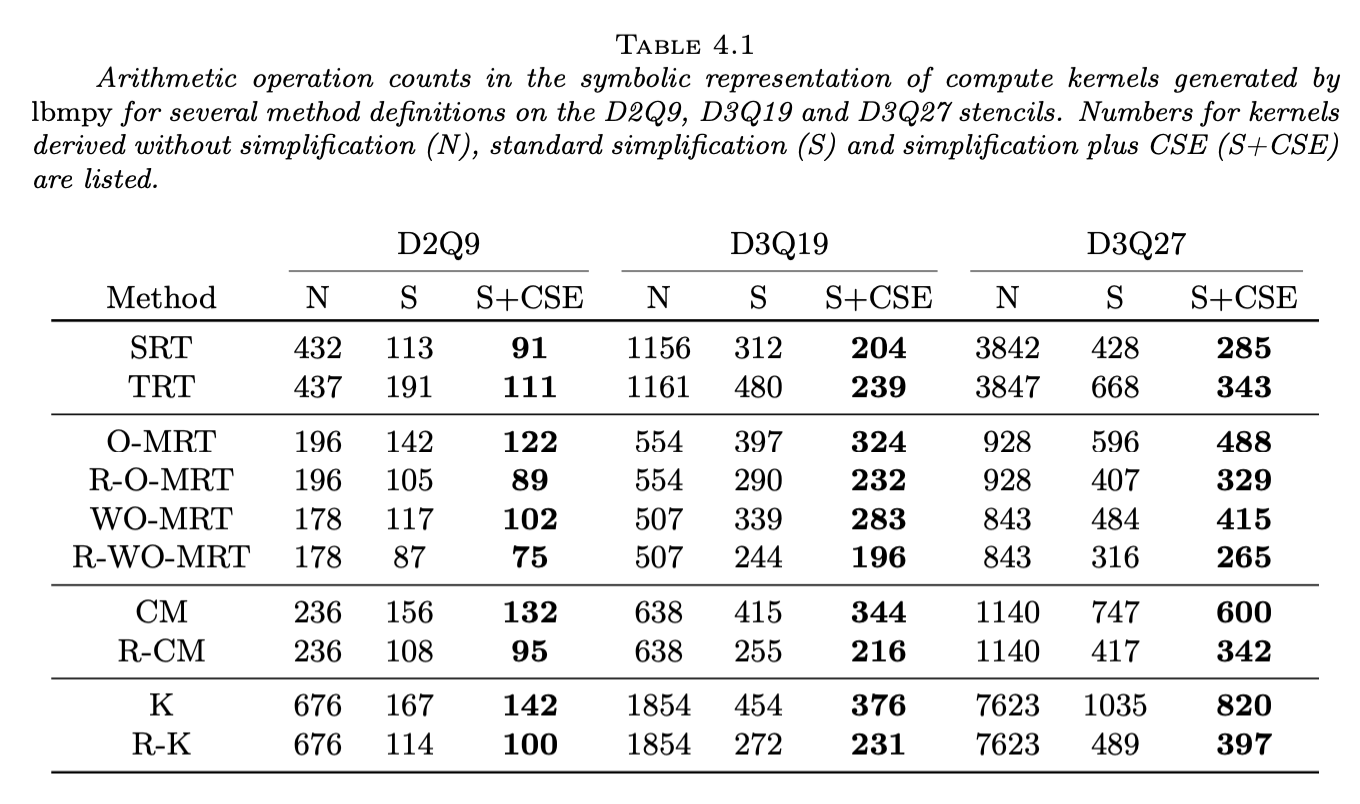
\includegraphics[width=0.8\linewidth]{arith_table.png}
  \end{center}
  For reference, my had \textsc{CM} implementation (slight over estimate) $220,702$ arithmetic operations.
  \blfootnote{From \cite{Hennig2023}}
\end{frame}





% Paper Conclusion
\begin{frame}{Paper Conclusion}
  \begin{outline}
  \1 \lstinline{lbmpy} now has SOTA collision spaces
  \2 Far more efficient than other implementations
  \1 High level symbolic representation
  \2 Easy to experiment with variant methods
  \2 Easy to target alternate architectures
  \1 Easy to scale with waLBerla
\end{outline}
\end{frame}


\section{Future Work}\label{sec:futurework}
\subsection{Tracer Particles}
Mentioned in my original proposal, tracer particles
represent a powerful tool for creating visual effects.
In reality, we mostly visualize fluid flow via particles or
other objects that are carried by the fluid, like smoke or bubbles.
Utilizing tracer particles can help realize a more true-to-life
visual affect than visualizing, for example, velocity as we did in
figure \ref{fig:movie-frame}.
Using large numbers of tracer particles to generate a 
density field which is then rendered volumetrically was used to 
great effect in \cite{Li2020, Li2024, Lyu2021}.

\subsection{Zero-centered Storage}
Zero-centered storage extends the Galilean invariance of CM-MRT 
into the storage of our $f$ distributions.
It has been shown that $f_i$ don't deviate far from the reference
frame equilibrium.
By instead storing and operating on $\delta f = f - f_u$ 
we can greatly increase the numerical accuracy by better
utilizing the available bits of our floating point representation.
Zero-centered storage is thoroughly explained in \cite{Hennig2023}.
Zero-centered storage would also open the door for using a half-float 
based storage, which would be a significant improvement if viable.

\subsection{Error Aware Compiling}
Currently my code generation is quite naive, simply
templating the SymPy expressions into shader code.
However, this yeilds expressions with numerical instabilities.
For example, in summation operations it would be better to alternate
$+$ and $-$ terms in order to preserve floating point accuracy.
Symbolic manipulation improvements could lead to greater numerical 
accuracy.

\subsection{Domain Decomposition}
Right now our solver only works on a single continuous allocation
for the entire domain.
Allowing the domain to be split over many blocks would have several 
advantages.
\begin{itemize}
\item \textit{Utilizing Additional Memory } \\
My Macbook has a limit on storage buffer sizes of a little over $4$gb.
Domain decomposition would allow me to utilize more buffers, and thus more of the $64$gb I have available.

\item \textit{Distributed Computing} \\
Distributing the solve over several compute nodes would require 
domain decomposition. 
This could be multiple GPUs in one system or
multiple compute nodes in an HPC environment.

\item \text{Spatial Adaptivity} \\
Most exciting, domain decomposition would be 
the next step towards spatial adaptivity. 
Spatial adaptivity would allow the limited memory resources to
capture a greater amount of detail in turbulent flows.
\end{itemize}



\begin{frame}{Conclusion}
  \begin{outline}
  \1 Today we've introduced Taichi
  \2 Python based implementation
  \2 Design Goals
  \2 Applications and Research Projects
  \2 Sparse Data Structures
  \1 Questions?
  \end{outline}
\end{frame}



% Eh
% \begin{frame}
  \begin{outline}
   \1 \cite{Yu2025Filter}
  \end{outline}
\end{frame}


\begin{frame}[allowframebreaks]{References}
    \tiny
    \printbibliography
\end{frame}

\end{document}


